\setcounter{ex}{0}
\section{HỆ BẤT PHƯƠNG TRÌNH BẬC NHẤT MỘT ẨN}
    Tìm cực trị biểu thức \fbox{$F=ax+by$} trên một miền đa giác
    \begin{itemize}
        \item \textbf{Bước 1:} Đặt ẩn số phụ $x$ và $y$ tương ứng với các đại lượng đề bài cho.
        \item \textbf{Bước 2:} Thiết lập các điều kiện $x$ và $y$ và biểu thức cần tìm giá trị lớn nhất (hoặc nhỏ nhất) theo vào $x$ và $y$.
        \item \textbf{Bước 3:} Đặt tất cả các $x$ và $y$ là cùng một hệ. Biểu diễn miền nghiệm của hệ trên.
        \item \textbf{Bước 4:} Tìm toạ độ các đỉnh của miền nghiệm của hệ trên.
        \item \textbf{Bước 5:} Tính giá trị của biểu thức cần tìm giá trị lớn nhất (hoặc nhỏ nhất) tại các đỉnh của miền nghiệm rồi chọn giá trị lớn nhất (hoặc nhỏ nhất) theo yêu cầu của đề bài.
    \end{itemize}

\begin{khung4}
    {\damEX Bài toán (ĐỀ TNTHPT 2025)}
    Để gây quỹ từ thiện, câu lạc bộ thiện nguyện của một trường THPT tổ chức hoạt động bán hàng với hai mặt hàng là nước chanh và khoai chiên. Câu lạc bộ thiết kế hai thực đơn. Thực đơn $1$ có giá $30$ nghìn đồng, bao gồm hai cốc nước chanh và một túi khoai chiên. Thực đơn $2$ có giá $50$ nghìn đồng, bao gồm ba cốc nước chanh và hai túi khoai chiên. Biết rằng câu lạc bộ chỉ làm được không quá $165$ cốc nước chanh và $100$ túi khoai chiên. Số tiền lớn nhất mà câu lạc bộ có thể nhận được sau khi bán hết hàng bằng bao nhiêu nghìn đồng?
\end{khung4}
{\color{\mauLG}\damEX\strut\faCommenting\ Lời giải.}\\
        Gọi $x$, $y$ lần lượt là số thực đơn $1$ và thực đơn $2$ bán được.\\	
        Số tiền thu được là 
        $F(x;y)=30x+50y$ (nghìn đồng).\\
        Ta có hệ $\heva{&x\geq 0\\&y\geq 0\\&2x+3y\leq 165\\&x+2y\leq 100.} $\\
        \centerline{
            \begin{tikzpicture}[line join=round, line cap=round,>=stealth,yscale=0.5,xscale=0.5]
                \begin{scope}
                    \clip (-1,-1.5) rectangle (12,7);
                    \fill[pattern=north east lines] (-2,6)--(-2,7)--(12,7)--(12,-1);
                    \fill[pattern=north east lines] (-2,7)--(12,7)--(12,-2.5);
                    \fill[pattern=north east lines] (-2,0)--(-2,-2.5)--(12,-2.5)--(12,0);;
                    \fill[pattern=north east lines] (-2,0)--(-2,7)--(0,7)--(0,0);;
                    \draw (-2,6)--(12,-1) node [pos=0.65, above,black] {$d_1$};
                    \draw  (-2,41/6)--(12,-2.5);
                    \node at (10.3,-0.7) {$d_2$};
                \end{scope}
                \fill (8.25,0) circle (1.2pt); 
                \fill (0,5) circle (1.2pt) node[shift={(.2,-.3)}]{$50$};
                \draw[->] (-1,0)--(12,0) node[right]{$x$};
                \draw[->] (0,-1)--(0,7) node[left]{$y$};
                \draw (0,0) node[below left]{$O$}  (0,4.5)node[left]{$C$} (10,0)node[above]{$100$}   ;
                \draw[dashed](3,0)node[below]{$30$}--(3,3.5)node[above]{$B$}--(0,3.5)node[left]{$35$} (8.25,0)node[below,xshift=-10pt]{$82{,}5$}
                (8.25,0)node[above,xshift=-24pt]{$A$}
                ;
            \end{tikzpicture}
        }
        Miền nghiệm là miền tứ giác $OABC$	trên hình vẽ kể cả các cạnh của tứ giác.\\
        Với các điểm cực biên là 
        $O(0;0)$, $A(82{,}5;0)$, $B(30;35)$, $C(0;50)$.\\
        Ta có $F(0;0)=0$; $F(82{,}5;0)=2\,475$; $F(30;35)=2\,650$; $F(0;50)=2\,500$.\\	
        Số tiền lớn nhất mà câu lạc bộ có thể nhận được sau khi bán hết hàng là 
        $2\,650$ nghìn đồng.		

\Opensolutionfile{ans}[ans/DA-CD6-HE-BPT-BTRL]
\subsection{Bài tập rèn luyện}

\begin{ex}%[0D3N1-2]
    Cặp số nào sau đây là nghiệm của hệ bất phương trình  $\heva{& x+2y\le8\\ & 3x-y>3 }$ ?
    \choice
    {$\left(0; 4\right)$ }
    {$\left(1; -1\right)$}
    {\True $\left(4; 1\right)$}
    {$\left(2; 3\right)$}
   \loigiai{
       Lần lượt thay các bộ số vào hệ bất phương trình ta được một nghiệm của hệ bất phương trình trên là $\left(4; 1\right)$.
   }
\end{ex}	

\begin{ex}%[0D3N1-2]
    Cho hệ bất phương trình $\heva{& x+3y-2\ge0\\ & 2x+y+1\le0 }$. Trong các điểm sau, điểm nào thuộc miền nghiệm của hệ bất phương trình?
    \choice
    {$M\left(0;1\right)$}
    {\True $N\left(-1;1\right)$}
    {$P\left(1;3\right)$}
    {$Q\left(-1;0\right)$}
   \loigiai{
       Ta thay lần lượt tọa độ các điểm vào hệ bất phương trình.\\
       Ta thấy $N\left(-1;1\right)$ thỏa mãn.
   }
\end{ex}

\begin{ex}%[0D3N1-2]
    Miền nghiệm của hệ bất phương trình $\heva{& x-2y+2>0\\ & 2x+y>3 }$  là phần mặt phẳng chứa điểm
    \choice
    {$\left(1;1\right)$ }
    {$\left(-1;2\right)$}
    {$\left(2;-1\right)$}
    {\True $\left(1;2\right)$}
   \loigiai{
       Lần lượt thay các bộ số vào hệ bất phương trình ta được một nghiệm của hệ bất phương trình trên là  $\left(1;2\right)$.
   }
\end{ex}	

\begin{ex}%[0D2H2-2]
    \immini[thm]{
        Phần \textbf{không tô đậm} trong hình vẽ bên (không chứa biên), biểu diễn tập nghiệm của hệ bất phương trình nào trong các hệ bất phương trình sau?
        \choice
        {$\heva{& x-y\ge 0 \\& 2x-y\ge 1}$}
        {\True $\heva{& x-y>0 \\& 2x-y>1}$}
        {$\heva{& x-y<0 \\& 2x-y>1}$}
        {$\heva{& x-y<0 \\& 2x-y<1}$}
    }
    {
        \begin{tikzpicture}[line join=round, line cap=round, >=stealth,font=\footnotesize, scale=0.7]
            \draw[->](-2,0)--(3,0) node[below right] {$x$};
            \draw[->](0,-3)--(0,3) node[above] {$y$};
            \clip (-2,-3) rectangle (3,3);
            \node (0,0) [above left]{$ O $};
            \foreach \x in {-1,...,2}
            \draw[shift={(\x,0)},color=black] (0pt,2pt) -- (0pt,-2pt);
            \foreach \y in {-1,...,3}
            \draw[shift={(0,\y)},color=black] (2pt,0pt) -- (-2pt,0pt);
            \draw[samples=100,smooth,domain=-4:2] plot(\x,{(\x)});
            \draw[samples=100,smooth,domain=-4:2] plot(\x,{2*(\x)-1});
            \draw [pattern=north west lines] (3,3)--(-2,3)--(-2,-3)--(-1,-3)--(1,1)--cycle;
            \draw[dashed] (0,1)--(1,1)--(1,0);
            \draw (0,1) node[left]{$1$} (1,0) node[below]{$1$} (0,-1) node[left]{$-1$};
        \end{tikzpicture}
    }
    \loigiai
    {
        Do miền nghiệm không chứa biên nên ta loại đáp án $\heva{& x-y\ge 0 \\& 2x-y\ge 1.}$\\
        Chọn điểm $M(1;0)$ thử vào các hệ bất phương trình.\\
        Xét đáp án $\heva{& x-y>0 \\& 2x-y>1}$, ta có $\heva{& 1-0>0 \\& 2\cdot 1-0>1}$ (luôn đúng) và miền nghiệm không chứa biên.
    }
    \dotlineEX{1}% Tạo các dòng kẻ trong tài liệu
\end{ex}


\begin{ex}%[0D2H2-2]
    \immini[thm]{
        Phần \textbf{không tô đậm} trong hình vẽ bên (không chứa biên), biểu diễn tập nghiệm của hệ bất phương trình nào trong các hệ bất phương trình sau?
        \choice
        {$\heva{& x-2y\le 0 \\& x+3y\ge -2}$}
        {$\heva{& x-2y>0 \\& x+3y<-2}$}
        {$\heva{& x-2y\le 0 \\& x+3y\le -2}$}
        {\True $\heva{& x-2y<0 \\& x+3y>-2}$}
    }
    {
        \begin{tikzpicture}[line join=round, line cap=round, >=stealth,font=\footnotesize, scale=0.8]
            \draw[->](-3,0)--(3,0) node[below right] {$x$};
            \draw[->](0,-2)--(0,2) node[above] {$y$};
            \clip (-3,-2) rectangle (3,2);
            \node (0,0) [above left]{$ O $};
            \foreach \x in {-2,...,2}
            \draw[shift={(\x,0)},color=black] (0pt,2pt) -- (0pt,-2pt);
            \foreach \y in {-1,...,1}
            \draw[shift={(0,\y)},color=black] (2pt,0pt) -- (-2pt,0pt);
            \draw[samples=100,smooth,domain=-3:3] plot(\x,{(\x)/2});
            \draw[samples=100,smooth,domain=-3:3] plot(\x,{(-(\x)-2)/3});
            \draw [pattern=north east lines] (-3,1/3)--(-3,-2)--(3,-2)--(3,3/2)--(-0.8,-0.4)--cycle;
            \draw[dashed] (0,1)--(2,1)--(2,0);
            \draw (0,1) node[left]{$1$} (2,0) node[below]{$2$} (-2,0) node[above]{$-2$};
        \end{tikzpicture}
    }
    \loigiai
    {
        Do miền nghiệm không chứa biên nên ta loại đáp án $\heva{& x-2y\le 0 \\& x+3y\ge -2}$ và $\heva{& x-2y\le 0 \\& x+3y\le -2.}$\\
        Chọn điểm $M(0;1)$ thử vào các hệ bất phương trình.\\
        Xét đáp án $\heva{& x-2y<0 \\& x+3y>-2}$, ta có $\heva{& 0-2\cdot 1>0 \\& 0+3\cdot 1>-2 }$ (luôn đúng) và miền nghiệm không chứa biên.
    }
    \dotlineEX{1}% Tạo các dòng kẻ trong tài liệu
\end{ex}



\begin{ex}%[0D2H2-2]
    Miền nghiệm của hệ bất phương trình $\heva{& x+y-1>0\\ & y\geq 2\\ &-x+2y>3}$ là phần \textbf{không} tô đậm của hình vẽ nào trong các hình vẽ sau?
    \choice
    {\begin{tikzpicture}[line join=round, line cap=round, >=stealth,font=\footnotesize, scale=0.4]
            % Vẽ hệ trục toạ độ
            \draw (0,0) node [below left] {$O$};
            \draw [->] (-3.5,0)--(3.5,0) node[below]{$x$};
            \draw[->] (0,-3.5)--(0,3.5) node[left]{$y$};
            \clip(-3.5,-3.5) rectangle (3.5,3.5);
            % Vẽ các số trên hai trục
            \foreach \x in {-3,1}
            \draw[shift={(\x,0)},color=black] (0pt,2pt) -- (0pt,-2pt) node[below] {\footnotesize $\x$};
            \foreach \y in {1,2}
            \draw[shift={(0,\y)},color=black] (2pt,0pt) -- (-2pt,0pt)node[left] {\footnotesize $\y$};
            %Vẽ đồ thị từng hàm số
            \draw[samples=100,smooth,domain=-3.5:3.5,black] plot(\x,{2});
            \draw[samples=100,smooth,domain=-3.5:3.5,black] plot(\x,{1-(\x)});
            \draw[samples=100,smooth,domain=-3.5:3.5,black] plot(\x,{0.5*(\x)+1.5});
            % Vẽ miền nghiệm
            \fill[pattern=north east lines,opacity=0.6] plot[domain=-3.5:3.5](\x,{1-(\x)})--plot[domain=3.5:-3.5](\x,{-3.5})--cycle;
            \fill[pattern=north east lines,opacity=0.6] plot[domain=-3.5:3.5](\x,{2})--plot[domain=3.5:-3.5](\x,{-3.5})--cycle;
            \fill[pattern=north east lines,opacity=0.6] plot[domain=-3.5:3.5](\x,{0.5*(\x)+1.5})--plot[domain=3.5:-3.5](\x,{3.5})--cycle;
    \end{tikzpicture}}
    {\True\begin{tikzpicture}[line join=round, line cap=round, >=stealth,font=\footnotesize, scale=0.4]
            % Vẽ hệ trục toạ độ
            \draw (0,0) node [below left] {$O$};
            \draw [->] (-3.5,0)--(3.5,0) node[below]{$x$};
            \draw[->] (0,-3.5)--(0,3.5) node[left]{$y$};
            \clip(-3.5,-3.5) rectangle (3.5,3.5);
            % Vẽ các số trên hai trục
            \foreach \x in {-3,1}
            \draw[shift={(\x,0)},color=black] (0pt,2pt) -- (0pt,-2pt) node[below] {\footnotesize $\x$};
            \foreach \y in {1,2}
            \draw[shift={(0,\y)},color=black] (2pt,0pt) -- (-2pt,0pt)node[left] {\footnotesize $\y$};
            %Vẽ đồ thị từng hàm số
            \draw[samples=100,smooth,domain=-3.5:3.5,black] plot(\x,{2});
            \draw[samples=100,smooth,domain=-3.5:3.5,black] plot(\x,{1-(\x)});
            \draw[samples=100,smooth,domain=-3.5:3.5,black] plot(\x,{0.5*(\x)+1.5});
            % Vẽ miền nghiệm
            \fill[pattern=north east lines,opacity=0.6] plot[domain=-3.5:3.5](\x,{1-(\x)})--plot[domain=3.5:-3.5](\x,{-3.5})--cycle;
            \fill[pattern=north east lines,opacity=0.6] plot[domain=-3.5:3.5](\x,{2})--plot[domain=3.5:-3.5](\x,{-3.5})--cycle;
            \fill[pattern=north east lines,opacity=0.6] plot[domain=-3.5:3.5](\x,{0.5*(\x)+1.5})--plot[domain=3.5:-3.5](\x,{-3.5})--cycle;
    \end{tikzpicture}}
    {\begin{tikzpicture}[line join=round, line cap=round, >=stealth,font=\footnotesize, scale=0.4]
            % Vẽ hệ trục toạ độ
            \draw (0,0) node [below left] {$O$};
            \draw [->] (-3.5,0)--(3.5,0) node[below]{$x$};
            \draw[->] (0,-3.5)--(0,3.5) node[left]{$y$};
            \clip(-3.5,-3.5) rectangle (3.5,3.5);
            % Vẽ các số trên hai trục
            \foreach \x in {-3,1}
            \draw[shift={(\x,0)},color=black] (0pt,2pt) -- (0pt,-2pt) node[below] {\footnotesize $\x$};
            \foreach \y in {1,2}
            \draw[shift={(0,\y)},color=black] (2pt,0pt) -- (-2pt,0pt)node[left] {\footnotesize $\y$};
            %Vẽ đồ thị từng hàm số
            \draw[samples=100,smooth,domain=-3.5:3.5,black] plot(\x,{2});
            \draw[samples=100,smooth,domain=-3.5:3.5,black] plot(\x,{1-(\x)});
            \draw[samples=100,smooth,domain=-3.5:3.5,black] plot(\x,{0.5*(\x)+1.5});
            % Vẽ miền nghiệm
            \fill[pattern=north east lines,opacity=0.6] plot[domain=-3.5:3.5](\x,{1-(\x)})--plot[domain=3.5:-3.5](\x,{3.5})--cycle;
            \fill[pattern=north east lines,opacity=0.6] plot[domain=-3.5:3.5](\x,{2})--plot[domain=3.5:-3.5](\x,{-3.5})--cycle;
            \fill[pattern=north east lines,opacity=0.6] plot[domain=-3.5:3.5](\x,{0.5*(\x)+1.5})--plot[domain=3.5:-3.5](\x,{-3.5})--cycle;
    \end{tikzpicture}}
    {\begin{tikzpicture}[line join=round, line cap=round, >=stealth,font=\footnotesize, scale=0.4]
            % Vẽ hệ trục toạ độ
            \draw (0,0) node [below left] {$O$};
            \draw [->] (-3.5,0)--(3.5,0) node[below]{$x$};
            \draw[->] (0,-3.5)--(0,3.5) node[left]{$y$};
            \clip(-3.5,-3.5) rectangle (3.5,3.5);
            % Vẽ các số trên hai trục
            \foreach \x in {-3,1}
            \draw[shift={(\x,0)},color=black] (0pt,2pt) -- (0pt,-2pt) node[below] {\footnotesize $\x$};
            \foreach \y in {1,2}
            \draw[shift={(0,\y)},color=black] (2pt,0pt) -- (-2pt,0pt)node[left] {\footnotesize $\y$};
            %Vẽ đồ thị từng hàm số
            \draw[samples=100,smooth,domain=-3.5:3.5,black] plot(\x,{2});
            \draw[samples=100,smooth,domain=-3.5:3.5,black] plot(\x,{1-(\x)});
            \draw[samples=100,smooth,domain=-3.5:3.5,black] plot(\x,{0.5*(\x)+1.5});
            % Vẽ miền nghiệm
            \fill[pattern=north east lines,opacity=0.6] plot[domain=-3.5:3.5](\x,{1-(\x)})--plot[domain=3.5:-3.5](\x,{3.5})--cycle;
            \fill[pattern=north east lines,opacity=0.6] plot[domain=-3.5:3.5](\x,{2})--plot[domain=3.5:-3.5](\x,{3.5})--cycle;
            \fill[pattern=north east lines,opacity=0.6] plot[domain=-3.5:3.5](\x,{0.5*(\x)+1.5})--plot[domain=3.5:-3.5](\x,{-3.5})--cycle;
    \end{tikzpicture}}
    \loigiai{
        Chọn điểm $(0;3)$ là điểm nằm trong miền nghiệm hệ bất phương trình. Do đó ta chọn hình 
        \begin{center}
            \begin{tikzpicture}[line join=round, line cap=round, >=stealth,font=\footnotesize, scale=0.6]
                % Vẽ hệ trục toạ độ
                \draw (0,0) node [below left] {$O$};
                \draw [->] (-3.5,0)--(3.5,0) node[below]{$x$};
                \draw[->] (0,-3.5)--(0,3.5) node[left]{$y$};
                \clip(-3.5,-3.5) rectangle (3.5,3.5);
                % Vẽ các số trên hai trục
                \foreach \x in {-3,1}
                \draw[shift={(\x,0)},color=black] (0pt,2pt) -- (0pt,-2pt) node[below] {\footnotesize $\x$};
                \foreach \y in {1,2}
                \draw[shift={(0,\y)},color=black] (2pt,0pt) -- (-2pt,0pt)node[left] {\footnotesize $\y$};
                %Vẽ đồ thị từng hàm số
                \draw[samples=100,smooth,domain=-3.5:3.5,black] plot(\x,{2});
                \draw[samples=100,smooth,domain=-3.5:3.5,black] plot(\x,{1-(\x)});
                \draw[samples=100,smooth,domain=-3.5:3.5,black] plot(\x,{0.5*(\x)+1.5});
                % Vẽ miền nghiệm
                \fill[pattern=north east lines,opacity=0.6] plot[domain=-3.5:3.5](\x,{1-(\x)})--plot[domain=3.5:-3.5](\x,{-3.5})--cycle;
                \fill[pattern=north east lines,opacity=0.6] plot[domain=-3.5:3.5](\x,{2})--plot[domain=3.5:-3.5](\x,{-3.5})--cycle;
                \fill[pattern=north east lines,opacity=0.6] plot[domain=-3.5:3.5](\x,{0.5*(\x)+1.5})--plot[domain=3.5:-3.5](\x,{-3.5})--cycle;
            \end{tikzpicture}
        \end{center}
    }	
\end{ex}


\begin{ex}%[0D2B2-2]
    \immini[thm]{   Miền tam giác $A B C$ kể cả ba cạnh sau đây là miền nghiệm của hệ bất phương trình nào trong bốn hệ bất phương trình dưới đây?
     \choice
    {$\heva{
            & y \geq 0 \\
            & 5 x-4 y \geq 10 \\
            & 5 x+4 y \leq 10
        }$}
    {$\heva{
            & x>0 \\
            & 5 x-4 y \leq 10 \\
            & 4 x+5 y \leq 10
        }$} 
    {$\heva{
            & x \geq 0 \\
            & 4 x-5 y \leq 10 \\
            & 5 x+4 y \leq 10
        }$}
    {\True $\heva{
            & x \geq 0 \\
            & 5 x-4 y \leq 10 \\
            & 4 x+5 y \leq 10
        }$}
    }
    {\begin{tikzpicture}[scale=0.8,yscale=.6,thick,>=stealth']
            %\fill[thin,color=gray!50] (-1,3.5) -- (4,3.5) -- (4,-1.2) -- (-1,2.8) -- cycle;
            %\fill[thin,color=gray!50] (-0.4,-3) -- (91/41,10/41) -- (4,-1.2) -- (4,-3) -- cycle;
            %\fill[thin,color=gray!50] (-1,2.8) -- (0,2) -- (0,-3) -- (-0.4,-3) --(-1,-3) -- cycle;
            \fill[thin,color=gray!50] (0,2) -- (0,-2.5) -- (91/41,10/41)  -- cycle;
            \draw[->] (-1,0) -- (4,0)node[above right]{$x$};
            \foreach \x in {1,2,3}
            \draw[shift={(\x,0)},color=black] (0pt,2pt) -- (0pt,-2pt) node[below] {\footnotesize $\x$};
            \draw[->,color=black] (0,-3) -- (0,3.5)node[above right]{$y$};
            \node[below right] at (0,0){$O$};
            \clip(-1,-3) rectangle (4,3.5);
            \draw[line width=1.2pt,smooth,samples=100,domain=-1:4] plot(\x,{5/4*(\x)-10/4});
            \draw[line width=1.2pt,smooth,samples=100,domain=-1:4] plot(\x,{10/5-4/5*(\x)});
            \foreach \y in {1,2,3}
            \draw[shift={(0,\y)},color=black] (2pt,0pt) -- (-2pt,0pt) node[left]{\footnotesize $\y$};
            \path 
            (0,2) coordinate (A)
            (90/41,10/41) coordinate (B)
            (0,-2.5) coordinate (C)
            ;
            \foreach \x/\g in {A/60,B/90,C/-10}
            \draw[fill=black] (\x) circle (.036)+(\g:.35)
            node{$\x$};	
            \draw[shift={(2.5,0)},color=black] (0pt,2pt) -- (0pt,-2pt) node[below] {\footnotesize $\frac{5}{2}$};
    \end{tikzpicture}}
    \loigiai{Cạnh $A C$ có phương trình $x=0$ và cạnh $A C$ nằm trong miền nghiệm nên $x \geq 0$ là một bất phương trình của hệ.\\[0.15cm]
        Cạnh $A B$ qua hai điểm $\left(\dfrac{5}{2} ; 0\right)$ và $(0 ; 2)$ nên có phương trình: $\dfrac{x}{\dfrac{5}{2}}+\dfrac{y}{2}=1 \Leftrightarrow 4 x+5 y=10$.\\[0.15cm]
        Vậy hệ bất phương trình cần tìm là $\heva{
            & x \geq 0 \\
            & 5 x-4 y \leq 10 \\
            & 4 x+5 y \leq 10
        }$.
    }
    \dotlineEX{4}% Tạo các dòng kẻ trong tài liệu
\end{ex}


\begin{ex}%[0D3N1-2]
    \immini[thm]{    Cho hệ bất phương trình $\heva{&-2x+y\le 2 \\ & -x+2y\ge 4 \\ & x+y\ge 5.}$   có miền nghiệm là miền được tô màu (miền tam giác $ABC$  có tọa độ các đỉnh là $A\left(2;0\right)$, $B\left(2;3\right)$, $C\left(1;4\right)$, bao gồm cả các cạnh) như hình vẽ: Giá trị nhỏ nhất $F_{\min}$  của biểu thức $F\left(x; y\right)$  trên miền xác định bởi hệ trên là 
        \choice
        {\True $F_{\min}=1$}
        {$F_{\min}=2$}
        {$F_{\min}=3$}
        {$F_{\min}=4$ }}{
        \begin{tikzpicture}[line join=round, line cap=round, >=stealth,font=\footnotesize, scale=0.6]
            % Vẽ hệ trục toạ độ
            \draw (0,0) node [below left] {$O$};
            \draw (0,2) node [below right] {$A$};
            \draw (1,4) node [above] {$B$};
            \draw (2,3) node [above] {$C$};
            \draw [->] (-2,0)--(4.5,0) node[below]{$x$};
            \draw[->] (0,-1)--(0,6) node[left]{$y$};
            \clip(-2,-1) rectangle (4.5,6);
            % Vẽ các số trên hai trục
            \foreach \x in {1,2}
            \draw[shift={(\x,0)},color=black] (0pt,2pt) -- (0pt,-2pt) node[below] {\footnotesize $\x$};
            \foreach \y in {2,3,4,5}
            \draw[shift={(0,\y)},color=black] (2pt,0pt) -- (-2pt,0pt)node[left] {\footnotesize $\y$};
            %Vẽ đồ thị từng hàm số
            \draw[samples=100,smooth,domain=-6.5:4.5,black] plot(\x,{2*(\x)+2});
            \draw[samples=100,smooth,domain=-6.5:4.5,black] plot(\x,{0.5*(\x)+2});
            \draw[samples=100,smooth,domain=-6.5:4.5,black] plot(\x,{-(\x)+5});
            % Vẽ miền nghiệm
            \fill[pattern=north west lines,opacity=0.6] (0,2)--(2,3)--(1,4)--cycle;
            \draw [dashed] (1,0)--(1,4)--(0,4) (2,0)--(2,3)--(0,3) ;
            \end{tikzpicture}}
    \loigiai{
        Tại $A\left(2;0\right)$ ta có:  $F\left(2;0\right)=2$.\\
        Tại $B\left(2;3\right)$  ta có: $F\left(2;3\right)=1$ .\\
        Tại $C\left(1;4\right)$  ta có:  $F\left(1;4\right)=3$.\\
        Vậy  $F_{\min}=1$.		
    }
\end{ex}

\begin{ex}[ĐH Vinh-Lần 1-2026]%[10D2K2-2]%[Dự án]
    Trong mặt phẳng toạ độ $Oxy$, gọi $(S)$ là miền nghiệm của hệ bất phương trình $\begin{cases} x + y \le 4 \\ 2x - y \ge 1 \\ x \ge 0 \\ y \ge 0. \end{cases}$
    \choiceTF
    {Điểm $A(1; 2)$ thuộc $(S)$}
    {\True $(S)$ là một miền tam giác}
    {Diện tích $(S)$ bằng $\frac{49}{6}$}
    { Giá trị lớn nhất của biểu thức $P = x+2y$ trên miền $(S)$ bằng $7$}
    \loigiai{
        Xác định miền nghiệm $(S)$ của hệ bất phương trình bằng cách vẽ các đường thẳng $d_1\colon x+y=4$ và $d_2\colon 2x-y=1$. 
        Giao điểm của các đường thẳng và các trục toạ độ tạo thành miền nghiệm $(S)$ là một tam giác với 3 đỉnh: 
        $M\left(\frac{1}{2}; 0\right)$, $N(4; 0)$ và $E\left(\frac{5}{3}; \frac{7}{3}\right)$.
        \begin{itemize}
            \item \textbf{Ý a) sai:} Thay toạ độ $A(1;2)$ vào bất phương trình thứ hai $2x-y \ge 1$ ta được $2(1) - 2 \ge 1 \Leftrightarrow 0 \ge 1$ (vô lý). Do đó, điểm $A$ không thuộc miền $(S)$.
            \item \textbf{Ý b) đúng:} Miền giới hạn $(S)$ là đa giác có 3 đỉnh $M, N, E$ như đã tìm ở trên, do đó nó là một miền tam giác.
            \item \textbf{Ý c) sai:} Tam giác có cạnh đáy $MN$ nằm trên trục $Ox$ với độ dài $MN = 4 - \frac{1}{2} = \frac{7}{2}$. Chiều cao hạ từ $E$ xuống $MN$ chính là tung độ của $E$, $h = \frac{7}{3}$. \\
            Diện tích $(S)$ là: $S_{\triangle MNE} = \frac{1}{2} \cdot MN \cdot h = \frac{1}{2} \cdot \frac{7}{2} \cdot \frac{7}{3} = \frac{49}{12}$.
            \item \textbf{Ý d) sai:} Ta tính giá trị của $P = x + 2y$ tại các đỉnh của miền $(S)$:
            \begin{itemize}
                \item Tại $M\left(\frac{1}{2}; 0\right) \Rightarrow P = \frac{1}{2}$.
                \item Tại $N(4; 0) \Rightarrow P = 4$.
                \item Tại $E\left(\frac{5}{3}; \frac{7}{3}\right) \Rightarrow P = \frac{5}{3} + 2\left(\frac{7}{3}\right) = \frac{19}{3}$.
            \end{itemize}
            Vậy giá trị lớn nhất của biểu thức $P$ trên miền $(S)$ bằng $\frac{19}{3}$.
        \end{itemize}
    }
    \dotlineEX{5}% Tạo các dòng kẻ trong tài liệu
\end{ex}
\begin{ex}%[10D2K2-2]%[Dự án]
    Bác Năm dự định trồng khoai lang và khoai mì trên mảnh đất có diện tích $8$ ha. Nếu trồng $1$ ha khoai lang thì cần $10$ ngày công và thu được $20$ triệu đồng. Nếu trồng $1$ ha khoai mì thì cần $15$ ngày công và thu được $25$ triệu đồng. Biết rằng, bác Năm chỉ có thể sử dụng được không quá $90$ ngày công cho công việc trồng khoai lang và khoai mì. Gọi $x, y$ lần lượt là số hecta trồng khoai lang và khoai mì. Các mệnh đề sau đúng hay sai?
    \choiceTF
    {\True Số tiền bác Năm thu về là $F(x, y) = 20x + 25y$ (triệu đồng)}
    {Hệ bất phương trình mô tả đầy đủ các điều kiện ràng buộc chỉ gồm $\begin{cases} x + y \le 8 \\ 10x + 15y \le 90 \end{cases}$}
    {Biểu diễn miền nghiệm của hệ bất phương trình các điều kiện ràng buộc là miền giới hạn bởi một tam giác (tính cả cạnh của tam giác)}
    {\True Số tiền nhiều nhất bác Năm có thể thu về được là $170$ triệu đồng}
    \loigiai{
        \begin{itemize}
            \item \textbf{Ý a) đúng:} Lợi nhuận thu được từ $x$ ha khoai lang và $y$ ha khoai mì là hàm mục tiêu $F(x; y) = 20x + 25y$.
            \item \textbf{Ý b) sai:} Để hệ ràng buộc đầy đủ ý nghĩa thực tế, cần bổ sung điều kiện không âm đối với diện tích đất trồng: $x \ge 0$ và $y \ge 0$.
            Hệ chuẩn phải là: $\begin{cases} x \ge 0 \\ y \ge 0 \\ x + y \le 8 \\ 10x + 15y \le 90 \end{cases} \Leftrightarrow \begin{cases} x \ge 0 \\ y \ge 0 \\ x + y \le 8 \\ 2x + 3y \le 18 \end{cases}$
            \item \textbf{Ý c) sai:} Vẽ miền nghiệm của hệ bất phương trình trên mặt phẳng $Oxy$, ta được miền giới hạn là một \textbf{tứ giác} có $4$ đỉnh với toạ độ lần lượt là: $O(0;0)$, $A(8;0)$, $B(6;2)$ và $C(0;6)$.
            \item \textbf{Ý d) đúng:} Thay toạ độ các đỉnh của tứ giác miền nghiệm vào hàm mục tiêu $F(x;y)$:
            \\ $F(0;0) = 0$
            \\ $F(8;0) = 20 \cdot 8 + 25 \cdot 0 = 160$
            \\ $F(0;6) = 20 \cdot 0 + 25 \cdot 6 = 150$
            \\ $F(6;2) = 20 \cdot 6 + 25 \cdot 2 = 170$
            \\ Vậy số tiền lớn nhất bác Năm có thể thu về là $170$ triệu đồng (khi trồng $6$ ha khoai lang và $2$ ha khoai mì).
        \end{itemize}
    }
    \dotlineEX{7}% Tạo các dòng kẻ trong tài liệu
\end{ex}

\begin{ex}%[10D2K2-2]%[Dự án]
    Một công ty TNHH trong một đợt quảng cáo và bán khuyến mãi hàng hóa cần thuê xe để chở ít nhất $140$ người và ít nhất $9$ tấn hàng. Nơi thuê chỉ có hai loại xe $A$ và $B$. Trong đó xe loại $A$ có $10$ chiếc, xe loại $B$ có $9$ chiếc. Một chiếc xe loại $A$ cho thuê với giá $4$ triệu đồng, loại $B$ giá $3$ triệu đồng. Biết rằng xe $A$ chỉ chở tối đa $20$ người và $0{,}6$ tấn hàng; xe $B$ chở tối đa $10$ người và $1{,}5$ tấn hàng. Gọi $x$ là số xe loại $A$ ($0 \le x \le 10; x \in \mathbb{N}$), $y$ là số xe loại $B$ ($0 \le y \le 9; y \in \mathbb{N}$). Các kết luận sau đúng hay sai?
    \choiceTF
    {\True Hàm mục tiêu thể hiện tổng chi phí thuê xe là $T = 4x + 3y$ (triệu đồng)}
    {\True Ràng buộc về số lượng người và số tấn hàng được mô tả bởi hệ $\begin{cases} 2x + y \ge 14 \\ 2x + 5y \ge 30 \end{cases}$}
    { Nếu bỏ qua điều kiện nguyên, miền biểu diễn tập nghiệm của hệ bất phương trình ràng buộc là một ngũ giác}
    {\True Để chi phí vận chuyển là thấp nhất, công ty cần thuê $5$ xe loại $A$ và $4$ xe loại $B$}
    \loigiai{
        \begin{itemize}
            \item \textbf{Ý a) đúng:} Tổng chi phí thuê $x$ xe loại A và $y$ xe loại B là $T(x; y) = 4x + 3y$.
            \item \textbf{Ý b) đúng:} 
            \\ Số người chở được: $20x + 10y \ge 140 \Leftrightarrow 2x + y \ge 14$.
            \\ Số tấn hàng chở được: $0{,}6x + 1{,}5y \ge 9 \Leftrightarrow 6x + 15y \ge 90 \Leftrightarrow 2x + 5y \ge 30$.
            \item \textbf{Ý c) sai:} Ta có hệ ràng buộc đầy đủ là $\begin{cases} 0 \le x \le 10 \\ 0 \le y \le 9 \\ 2x + y \ge 14 \\ 2x + 5y \ge 30 \end{cases}$. Vẽ trên hệ trục $Oxy$, miền nghiệm (bỏ qua điều kiện nguyên) là một \textbf{tứ giác} giới hạn bởi các đỉnh: $M(5;4)$, $N(10;2)$, $P(10;9)$ và $Q(2{,}5;9)$. Do đó đây không phải là ngũ giác.
            \item \textbf{Ý d) đúng:} Bài toán quy về tìm giá trị nhỏ nhất của $T = 4x + 3y$ trên miền nghiệm nguyên. Nhận thấy trong các đỉnh của miền nghiệm thực, điểm $M(5;4)$ có toạ độ nguyên. 
            \\ Ta thử nghiệm tại các đỉnh nguyên hoặc gần đỉnh:
            \\ Tại $M(5; 4) \Rightarrow T = 4(5) + 3(4) = 32$ (triệu đồng).
            \\ Tại $N(10; 2) \Rightarrow T = 4(10) + 3(2) = 46$ (triệu đồng).
            \\ Tại $P(10; 9) \Rightarrow T = 4(10) + 3(9) = 67$ (triệu đồng).
            \\ Xét một điểm nguyên khác nằm trong miền nghiệm, ví dụ $(4; 6) \Rightarrow T = 4(4) + 3(6) = 34 > 32$.
            \\ Vậy chi phí nhỏ nhất là $32$ triệu đồng khi thuê $5$ xe loại A và $4$ xe loại B.
        \end{itemize}
    }
    \dotlineEX{7}% Tạo các dòng kẻ trong tài liệu
\end{ex}
\begin{ex}[BGD2025]%[0D2V2-3]
    Để gây quỹ từ thiện, câu lạc bộ thiện nguyện của một trường THPT tổ chức hoạt động bán hàng với hai mặt hàng là nước chanh và khoai chiên. Câu lạc bộ thiết kế hai thực đơn. Thực đơn $1$ có giá $30$ nghìn đồng, bao gồm hai cốc nước chanh và một túi khoai chiên. Thực đơn $2$ có giá $50$ nghìn đồng, bao gồm ba cốc nước chanh và hai túi khoai chiên. Biết rằng câu lạc bộ chỉ làm được không quá $165$ cốc nước chanh và $100$ túi khoai chiên. Số tiền lớn nhất mà câu lạc bộ có thể nhận được sau khi bán hết hàng bằng bao nhiêu nghìn đồng?
    \shortans{$2650$}
    \loigiai{
        Gọi $x$, $y$ lần lượt là số thực đơn $1$ và thực đơn $2$ câu lạc bộ bán được.\\	
        Số tiền thu được là 
        $F(x;y)=30x+50y$ (nghìn đồng).\\
        Ta có hệ $\heva{&x\geq 0\\&y\geq 0\\&2x+3y\leq 165\\&x+2y\leq 100.} $\\
        Vẽ $d_1\colon x+2y=100$, $d_2\colon 2x+3y=165$.\\
        \begin{center}
            \begin{tikzpicture}[line join=round, line cap=round,>=stealth,yscale=0.5,xscale=0.5]
                \tikzset{label style/.style={font=\footnotesize}}
                \begin{scope}
                    \clip (-1,-1.5) rectangle (12,7);
                    \fill[pattern=north east lines] (-2,6)--(-2,7)--(12,7)--(12,-1);
                    \fill[pattern=north east lines] (-2,7)--(12,7)--(12,-2.5);
                    \fill[pattern=north east lines] (-2,0)--(-2,-2.5)--(12,-2.5)--(12,0);;
                    \fill[pattern=north east lines] (-2,0)--(-2,7)--(0,7)--(0,0);;
                    \draw (-2,6)--(12,-1) node [pos=0.65, above,rotate=-30] {$d_1$};
                    \draw (-2,41/6)--(12,-2.5);
                    \node at (10.3,-0.7) {$d_2$};
                \end{scope}
                \fill (8.25,0) circle (1.2pt); 
                \fill (0,5) circle (1.2pt) node[shift={(.2,-.3)}]{$50$};
                \draw[->] (-1,0)--(12,0) node[right]{$x$};
                \draw[->] (0,-1)--(0,7) node[left]{$y$};
                \draw (0,0) node[below left]{$O$}  (0,4.5)node[left]{$C$} (10,0)node[above]{$100$}   ;
                \draw[dashed](3,0)node[below]{$30$}--(3,3.5)node[above]{$B$}--(0,3.5)node[left]{$35$} (8.25,0)node[below,xshift=-10pt]{$82{,}5$}
                (8.25,0)node[above,xshift=-24pt]{$A$}
                ;
            \end{tikzpicture}		
        \end{center}
        Miền nghiệm là miền tứ giác $OABC$	trên hình vẽ kể cả các cạnh của tứ giác. Với các điểm cực biên là 
        $O(0;0)$, $A(82{,}5;0)$, $B(30;35)$, $C(0;50)$.\\
        Ta có $F(0;0)=0$; $F(82{,}5;0)=2\,475$; $F(30;35)=2\,650$; $F(0;50)=2\,500$.\\	
        Số tiền lớn nhất mà câu lạc bộ có thể nhận được sau khi bán hết hàng là 
        $2\,650$ nghìn đồng.		
    }
       \dotlineEX{7}% Tạo các dòng kẻ trong tài liệu
\end{ex}


\begin{ex}%[0D3N1-3]
    Một công ty điện tử sản xuất hai kiểu radio trên hai dây chuyền độc lập. Radio kiểu một sản xuất trên dây chuyền một với công suất  $45$ radio/ngày, radio kiểu hai sản xuất trên dây chuyền hai với công suất $80$  radio/ngày. Để sản xuất một chiếc radio kiểu một cần $12$  linh kiện, để sản xuất một chiếc radio kiểu hai cần $9$ linh kiện. Tiền lãi khi bán một chiếc radio kiểu một là $250000$  đồng, lãi thu được khi bán một chiếc radio kiểu hai là $180000$ đồng. Biết rằng số linh kiện có thể sử dụng tối đa trong một ngày là $900$. Gọi $x_0$, $y_0$  lần lượt là số radio kiểu một và radio kiểu hai sản suất được trong một ngày để tiền lãi thu được là nhiều nhất. Khi đó tổng $T=x_0+2y_0$  bằng
    \shortans{$125$}
    \loigiai{
        Gọi $x$  và  $y$ lần lượt là số radio kiểu một và số radio kiểu hai mà công ty này sản xuất trong một ngày $\left(x,\, y \in \mathbb{N}^*\right)$.\\ 
        Số tiền lãi mà công ty này thu về hàng ngày là $P=250000x+180000y$  (đồng).\\
        Ta có hệ bất phương trình  $\heva{&12x+9y\leq 900\\&0\leq x\leq 45\\&0\leq y\leq 80}$.\\
        Bài toán trở thành tìm giá trị lớn nhất của biểu thức $P=250000x+180000y$  trên miền nghiệm của hệ bất phương trình $\heva{&12x+9y\leq 900\\&0\leq x\leq 45\\&0\leq y\leq 80}$.
        \begin{center}
            \begin{tikzpicture}[scale=0.6,thick,>=stealth']
                \draw[->] (-3,0) -- (10,0)node[above]{$x$};
                %\foreach \x in {1,2,3,4,5,6,7,8,9,10,11,11,12}\draw[shift={(\x,0)},color=black] (0pt,2pt) -- (0pt,-2pt) node[below] {\footnotesize $\x$};
                \draw[->,color=black] (0,-2) -- (0,11)node[right]{$y$};
                %\foreach \y in {1,2,3,4,5,6,7,8,9}\draw[shift={(0,\y)},color=black] (2pt,0pt) -- (-2pt,0pt) node[left] {\footnotesize $\y$};
                \node[below left] at (0,0) {$O$};
                \clip(-3,-2) rectangle (10,11);
                %\fill[pattern=north east lines] (-0.15,14.3) -- (-1,14.3) -- (-1,-1) -- (7.5,-1)-- cycle;
                \draw[line width=1.2pt,smooth,samples=100,domain=-1:9] plot(\x,{-(12/9)*(\x)+10});
                %\fill[pattern=north east lines] (-1,6.4)--(-1,-1)--(15.3,-1)--(15.3,-0.12)-- cycle;
                \draw[line width=1.2pt,smooth,samples=100,domain=-1:15.3] plot(\x,{8});
                %\fill[pattern=north east lines] (-1,9)--(-1,14.3) --(15.3,14.3)--(15.3,9)-- cycle;
                
                \fill[pattern=north east lines] (0,0)--(0,8) --(1.5,8)--(4.5,4)-- (4.5,0)-- cycle;
                \node[above right] at (4.5,0) {$A$};
                \node[below right] at (4.5,0) {$45$};\node[below] at (7.5,0) {$75$};
                \node[right] at (4.5,4) {$B$}; \node[below] at (1.5,0) {$15$};
                \node[below left] at (0,8) {$80$};
                \node[above right] at (1.5,8) {$C$};\node[left] at (0,4) {$40$};
                \node[left] at (0,10) {$100$};
                \node[above left] at (0,8) {$D$};
                \draw[dashed] (0,4)--(4.5,4)  (1.5,0)--(1.5,8);
                \draw[thick] (4.5,-2)--(4.5,11);
            \end{tikzpicture}
        \end{center}
        Miền nghiệm của hệ bất phương trình $\heva{&12x+9y\leq 900\\&0\leq x\leq 45\\&0\leq y\leq 80}$ là miền ngũ giác $OABCD$  trong đó  $O\left(0;0\right)$, $A\left(45;0\right)$,  $B\left(45;40\right)$,  $C\left(15;80\right)$, $D\left(0;80\right)$. \\     
        Tại $O\left(0;0\right)$ , ta có $P=250000\cdot0+180000\cdot0=0$.\\  
        Tại $A\left(45;0\right)$ ta có  $P=250000\cdot45+180000\cdot0=11250000$.\\
        Tại  $B\left(45;40\right)$ ta có $P=250000\cdot45+180000\cdot40=18450000$. \\
        Tại  $C\left(15;80\right)$ ta có  $P=250000\cdot15+180000\cdot80=18150000$. 
        Tại $D\left(0;80\right)$  ta có  $P=250000\cdot0+180000\cdot80=14400000$. 
        Ta thấy biểu thức $P=250000x+180000y$   đạt giác trị lớn nhất khi $x_0=45, \, y_0=45$.\\
        Vậy $T=x_0+2y_0=125$.		
    }
    \dotlineEX{2}% Tạo các dòng kẻ trong tài liệu
\end{ex}
\begin{ex}[SỞ NINH BÌNH 25-26]
    Một công ty $A$ chuyên sản xuất giấy đã nhận được một đơn đặt hàng theo tháng từ đối tác $B$, mỗi tháng công ty $A$ phải cung cấp cho đối tác $B$ ít nhất $2800$ kg giấy in và $2400$ kg giấy carton. Công ty $A$ sử dụng hai loại nguyên liệu là gỗ keo và gỗ bạch đàn. Từ một tấn gỗ keo sản xuất ra được $200$ kg giấy in và $300$ kg giấy carton; từ một tấn gỗ bạch đàn sản xuất ra được $300$ kg giấy in và $150$ kg giấy carton. Một tấn gỗ keo có giá là $1,2$ triệu đồng và một tấn gỗ bạch đàn có giá là $1,5$ triệu đồng. Biết mỗi tháng cơ sở cung cấp nguyên liệu chỉ cung cấp không quá $9$ tấn gỗ keo và không quá $10$ tấn gỗ bạch đàn. Số tiền nhỏ nhất mà công ty $A$ cần dùng mỗi tháng để mua nguyên liệu là bao nhiêu triệu đồng?
    \shortans{15}
    \loigiai
    {
        Gọi số tấn gỗ keo mà công ty $A$ cần mua là $x$; số tấn gỗ bạch đàn công ty cần mua là $y$. Khi đó ta có:
        
        Điều kiện nguyên liệu: $0\leq x\leq 9$; $0\leq y\leq 10$.
        
        Khối lượng giấy in sản xuất được là $200x+300y$; điều kiện cần của khối lượng giấy in suy ra $200x+300y\geq 2800$.
        
        Khối lượng giấy carton sản xuất được là $300x+150y$; điều kiện cần của khối lượng giấy carton suy ra $300x+150y\geq 2400$.
        
        Chi phí mua nguyên liệu: $T=1,2x+1,5y$
        
        Biểu diễn miền nghiệm của hệ bất phương trình: $\begin{cases} 0\leq x\leq 9 \\ 0\leq y\leq 10 \\ 200x+300y\geq 2800 \\ 300x+150y\geq 2400\end{cases}$.
        
        \centerline{
            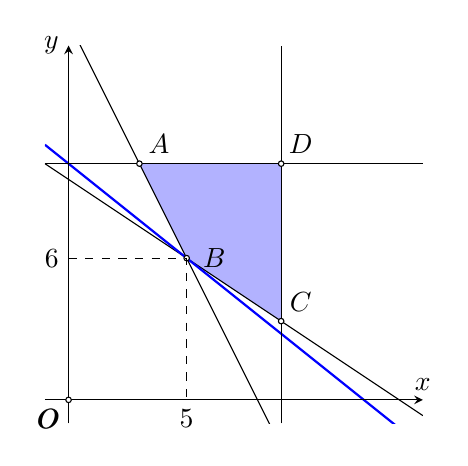
\begin{tikzpicture}[x=3mm,y=3mm]
                \path 
                (0,0) coordinate (O)
                (3,10) coordinate (A)
                (5,6) coordinate (B)
                (9,{10/3}) coordinate (C)
                (9,10) coordinate (D)
                ;
                \fill[blue!30] (A)--(B)--(C)--(D)--cycle;
                \begin{scope}
                    \clip (-1,-1) rectangle (15,15);
                    \draw[smooth] 
                    plot[domain=-1:15] (\x,{(-200*\x+2800)/300})
                    plot[domain=-1:15] (\x,{(-300*\x+2400)/150})
                    ;
                    \draw[smooth,blue,thick] plot[domain=-1:15](\x,{-0.8*\x+10});
                \end{scope}
                
                \draw (-1,10)--(15,10) (9,-1)--(9,15);
                \draw[-stealth] (-1,0)--(15,0) node[above]{$x$};
                \draw[-stealth] (0,-1)--(0,15) node[left]{$y$};
                \foreach \x/\g in {O/-135,A/45,B/0,C/45,D/45}\draw[fill=white] (\x) circle (1pt)+(\g:1em) node{$\x$};
                \draw[dashed] (0,6) node[left]{$6$}-|(5,0)node[below]{$5$} (0,0) node[below left]{$O$};
            \end{tikzpicture}
        }
        
        Miền nghiệm của hệ bất phương trình là phần tô màu trong hình vẽ trên, khi đó $T=1,2x+1,5y$ đạt giá trị nhỏ nhất tại một trong các đỉnh $B$ của đa giác miền nghiệm $ABCD$. Khi đó $T=15$ khi $x=5$; $y=6$.
    }
        \dotlineEX{2}% Tạo các dòng kẻ trong tài liệu
\end{ex}
\begin{ex}%[0D3N1-3]
    Gia đình chị Minh dự định trồng rau và hoa trên một mảnh đất có diện tích  $8$ ha. Nếu trồng $1$  ha rau thì cần $20$  ngày công và thu lợi $3$ triệu đồng. Nếu trồng $1$  ha hoa thì cần $30$  ngày công và thu lợi $4$  triệu đồng. Biết rằng, gia đình chị Minh chỉ có thể sử dụng không quá $180$  ngày công cho công việc trồng rau và hoa. Hỏi từ việc trồng rau và hoa nói trên, chị Minh có thể thu về lợi nhuận cao nhất là bao nhiêu triệu đồng.
    \shortans{$26$}
    \loigiai{
        Gọi $x, \, y\, \left(x\geq0, \,y\geq0\right)$    lần lượt là số ha đất trồng rau và hoa.\\
        Diện tích đất trồng canh tác không vượt quá $8$  ha nên ta có: $x+y\leq8$.\\  .
        Số ngày công sử dụng không vượt quá $180$ ngày nên $2x+3y\leq180$.\\
        Từ đó, ta có hệ bất phương trình: $\heva{&x+y\leq8\\&2x+3y\leq180\\&x\geq 0\\&y\geq 0}$\\ 
        Ta cần tìm  $x, \, y$   sao cho $T\left(x,y\right)=3x+4y$  lớn nhất.\\
        Miền nghiệm của hệ  được biểu diễn như sau:
        \begin{center}
            \begin{tikzpicture}[scale=0.6,thick,>=stealth']
                \draw[->] (-3,0) -- (12,0)node[above]{$x$};
                \foreach \x in {1,2,3,4,5,6,7,8,9,10,11}
                \draw[shift={(\x,0)},color=black] (0pt,2pt) -- (0pt,-2pt) node[below] {\footnotesize $\x$};
                \draw[->,color=black] (0,-2) -- (0,9)node[right]{$y$};
                \foreach \y in {1,2,3,4,5,6,7,8,9}
                \draw[shift={(0,\y)},color=black] (2pt,0pt) -- (-2pt,0pt) node[left] {\footnotesize $\y$};
                \node[below left] at (0,0) {$O$};
                \clip(-3,-2) rectangle (12,9);
                %\fill[pattern=north east lines] (-0.15,14.3) -- (-1,14.3) -- (-1,-1) -- (7.5,-1)-- cycle;
                \draw[line width=1.2pt,smooth,samples=100,domain=-3:9] plot(\x,{-(\x)+8});
                %\fill[pattern=north east lines] (-1,6.4)--(-1,-1)--(15.3,-1)--(15.3,-0.12)-- cycle;
                \draw[line width=1.2pt,smooth,samples=100,domain=-1:12] plot(\x,{-(2/3)*(\x)+6});			
                \fill[pattern=north east lines] (0,0)--(0,6) --(6,2)--(8,0)-- cycle;
                \node[above] at (8,0) {$A$};
                \node[right] at (6,2) {$B$};
                \node[right] at (0,6) {$C$};			
            \end{tikzpicture}
        \end{center}
        Miền nghiệm của hệ bất phương trình trên là miền trong của tứ giác $OABC$  , kể cả các  cạnh của tứ giác đó, với  $O\left(0;0\right)$, $A\left(8;0\right)$,  $B\left(6;2\right)$,  $C\left(0;6\right)$. \\
        Tại $O\left(0;0\right)$  , ta có: $T=3\cdot0+4\cdot0=0$.\\ 
        Tại $A\left(8;0\right)$ , ta có:  $T=3\cdot8+4\cdot0=24$.\\ 
        Tại $B\left(6;2\right)$ , ta có:  $T=3\cdot6+4\cdot2=26$.\\
        Tại $C\left(0;6\right)$ , ta có: $T=3\cdot0+4\cdot6=24$.\\ 
        Vậy số lợi nhuận cao nhất mà gia đình chị Minh thu được từ trồng rau và hoa là $26$ triệu đồng.	
    }
        \dotlineEX{2}% Tạo các dòng kẻ trong tài liệu
\end{ex}
\Closesolutionfile{ans}
%\inputansbox{10,5,5}{ans/DA-CD6-HE-BPT-BT}